\documentclass{article}
\setlength{\parindent}{0cm}
\setlength{\parskip}{5mm}
%\setlength{\topsep}{-1cm}
%\setlength{\itemsep}{-1cm}
\setlength{\oddsidemargin}{-.3in}
\setlength{\evensidemargin}{-.3in}
\setlength{\textwidth}{6.5in}
\setlength{\textheight}{8in}

\setlength{\parskip}{0pt}
\setlength{\parsep}{0pt}
\setlength{\headsep}{0pt}
%% \setlength{\topskip}{0pt}
%% \setlength{\topmargin}{0pt}
%% \setlength{\topsep}{0pt}
%% \setlength{\partopsep}{0pt}

\usepackage{graphicx}
\usepackage{amsmath,mathrsfs,amsthm,amssymb}
\usepackage{subfigure}
\title{Do LDA algorithms learn LDA models? }
\author{Andrew Gambardella, Victor Huang, Satish Rao, Di Wang, Chenyu Zhao}

\date{}

\newcommand{\mcf}{{\zeta}}
\newcommand{\norm}[1]{\lVert#1\rVert}

\begin{document}
\maketitle

\begin{abstract}
The Latent Dirichlet Allocation topic model has received enormous
attention as a method for extracting insight from documents and a wide
variety of other data sources.  Two interesting aspects in its application
are the effectiveness of learning algorithms, and the applicability to real
data.  In this paper, we primarily study the former but also apply some
of what we learn to the latter.

For a common view, we define a natural (for LDA) prediction task and
generate data according to the LDA model. We then evaluate a range of
algorithms, including one of our invention, on this generated data.
We characterize features of the generated data to help predict the
peformance of these algorithms.  We also run the algorithms on
some real world datasets. 

We find that the standard algorithms for LDA are quite poor compared
with principal components methods (latent semantic indexing or LSI)
and our new method with data generated from their model.  In contrast,
the LDA methods do perform better than principal components methods on
real world data, though, fall far short of nearest neighbor methods.
While the goal of topic modelling is not nessarily prediction, we
believe this study provides useful information about their use.

We note that it is ironic that the algorithms for LDA fail to beat LSI based
methods on their "LDA" data  but do on real world data.
\end{abstract}

\section{Introduction} \label{sec:intro}

With the vast production of data comes a great desire
to understand and make use of its structure. One
avenue has been to use generative models to provide
insight.  Topic models, in particular,
have been quite popular to investigate documents
and an increasing number of other domains (See \cite{BleiCACM} for
a survey of this field.)

% The early history of these things...

A relevant, prehistorical, viewpoint is the concept of latent semantic
indexing which views a document as being about a subset of a larger
set of topics.  Topics are in turn are about (positive numbers) or not
about (negative numbers) certain words \cite{Papadimitriou1997}.  They
used this view to provide an algorithm based on linear algebra that
learned the structure of their model.  They also argued that this
model provided some insight into the wide applicability of principal
components analysis in data analysis. The algorithmic tool at the
core of their work (and principal components) was the singular value
decomposition.

Shortly thereafter, a probabilistic framework was provided by Puzicha
and Hofmann \cite{Hofmann04}.  They termed their method probabilisitc latent
semantic indexing (pLSI), and modelled topics as probability
distributions over words (no negative numbers in this description).
Documents were then presumed to be generated as a mixture of these
topics.  The large number of parameters in the PLSI model motivated
Blei, Ng and Jordan to provide a generative model for these parameters
as well; they provided the enormously influential Latent Dirichlet
Allocation(LDA) topic model \cite{Blei2003a}.

Both pLSI and LDA have had enormous impact, but remain challenging
both in terms of the appropriateness of the model and in terms of
algorithms fitting the model.  The evaluation of efficacy departed
from tradition in machine learning in that one evaluated the learned
parameters in terms of predicted probability of the corpus
(``perplexity'') rather than on the performance of some task. Indeed,
this perspective remains compelling.  For example, in
\cite{BleiCBA} the evaluation of new algorithms still proceeds very
much using these internal measures.  This has merits in that one goal
of topic modelling is to find something ``interesting'', for which
performance is difficult to define.  Still, the form of the measures
suggested in the literature can be very complex.  See, for example, \cite{BleiCBA}.
 
This complexity can make it very difficult to see when such models are
appropriate or whether the algorithms are effectively learning the
model.  We repeat for emphasis that there are {\em two issues here}:
the applicability of the model, and the effectiveness of the
algorithm.  Neither is easy to evaluate in engineering the methods
for data analytics.

We seek to provide insight into the performance of algorithms and to
some extent understand the application to data.  In contrast to the
tendencies in topic modelling \cite{BleiCBA}, we wish to provide simple
methods for evaluation. In this paper, we primarily study the
effectiveness of algorithms for discerning LDA models {\em when we
know} they apply; for data generated by the model.

%%   We derive some
%% insights and discuss some real world datasets.  

An effective model should lead to good performance on prediction. We
thus return to a simple prediction task as a primary figure of merit.
Topic models, particularly LDA, generate documents word by word.
Thus, a fair evaluation is to use a training set of documents and a
subset of a document to predict an unseen word.  This task, as we
show, entails both learning the topics and the distribution of topics
in a particular document.  The ``one-more'' (or ``$k$-more'') word
task is central to our study.  This task also has natural
applications which we touch upon later.

A feature of this approach is that one can compare to methods not
based on modelling.  Thus, we can compare performance based on
modelling topics to standard learning methods.  In particular, we
include nearest neighbor methods which have been found to be highly
effective in the literature and in our experiments.

We found that for generated LDA data that the algorithms widely used for
learning LDA appear to be reasonably effective, but traditional
algorithms based on LSI are, in fact, {\em more effective.}  We
further engineered a new method combining LSI, $k$-means, and the
inference part of LDA.  This method is more robust than
LSI and has the best performance of any method we tested.

We characterize the instances that we can learn, the instances where
knowing the parameters give power (even when we fail to learn them),
and finally where the model fails to give any predictive advantage at
all even cheating.  The resulting characterization is unsuprising:
simply measure the independence or lack thereof of the selection of
words in a particular document is key.  On the other hand, taking
advantage of such simple measures has been key to giving provable
algorithms for numerous mixture problems ranging from learning
mixtures of Gaussians \cite{VempalaW04}, to hidden markov problems
\cite{MosselRoch}, to recent provable method for learning topic models
\cite{Arora2012} and even the LDA model \cite{AnandLDA}.  Indeed, we must
first recognize order before distinguishing it from chaos.

Finally, we test the methods on some real data sets.  Here, we find
that topic models do distinguish from chaos. Indeed, we find that the
LDA algorithms do better than both LSI and our engineered methods
which dominate on the simulated data.  This is quite interesting, and
gives gives testament to the notion that topic modellers have worked
extensively with real data; model or not.  Still, the most effective
algorithms in our experiments by far for real datasets is the nearest
neighbor algorithms.

To reiterate, the main study here is a simulation study to see whether
the modelling process produces better algorithms.  What appears to be
the case is that decent, though not champion, algorithms for real data
sets were developed for LDA despite them not being particularly good
for data generated by the actual model.  This suggests that the
algorithms may be more experimentally developed than formally
motivated.\footnote{We primarily report on a variational algorithm
for optimizing LDA.  We experimented with Gibbs Sampling
implementations as well as pLSI implementations.  The former was slow
but performed similarly to the variational approach, the latter
performed poorly.}  It remains quite interesting to characterize
what model is most appropriate for real world data, but 
understanding the relationship between algorithms and models
should be an important aspect of this. 

We proceed in the sequel by describing the LDA model in
section~\ref{sec:ldamodel}. We decribe the algorithms
in~\ref{sec:algs}. We give some experiments for a range of parameters
and for real datasets in section~\ref{sec:results}.  We explore the
border of where the algorithms and than even the topic
parameterization fail to provide performance in
section~\ref{sec:analysis}.  We conclude in
section~\ref{sec:conclusion}.







\section{Related work}
An early version of topic modeling is seen in Latent Semantic
Indexing (LSI) which views a document as a combination of a larger
set of topics.  Topics are in turn about certain words
(represented by positive numbers) or not about certain words
(represented by negative numbers) \cite{Papadimitriou1997}.  They
provided a linear algebra algorithm that learned the structure
of their model.  They also argued that this model provides
insight into the wide applicability of principal
components analysis in data analysis. The mathematical tool at the core
of their work (and PCA) was the singular value
decomposition.

Shortly thereafter, Puzicha and Hofmann \cite{Hofmann04} provided a
probabalistic framework, termed probabilisitc latent
semantic indexing (PLSI). Topics are modelled as probability
distributions over words (no negative numbers). Documents are
then assumed to be generated as a mixture of these
topics. 

The large number of parameters in the PLSI model motivated
Blei, Ng and Jordan to develop a generative model for these parameters,
which resulted in the enormously influential Latent Dirichlet
Allocation (LDA) topic model \cite{Blei2003a}.

The most closely related works in theory are the aforementioned
algorithms provided by Arora et.al. \cite{Arora2012} which learn PLSI
under certain assumptions, and a breakthrough by
Anandkumar~\cite{AnandLDA} which gives a provably convergent algorithm
for learning LDA with polynomial data requirements.  There is a long
literature in learning mixture models in statistics and
more recently in theoretical computer science. See
\cite{MoitraValiant} for a recent breakthrough on learning mixtures of
Gaussians and a discussion of this field.

There is ample work describing methods for optimizing
LDA \cite{BleiCACM}.  Recent examples are described
in \cite{McCallumMALLET}, \cite{BleiCBA}. 

There is also significant work on extending LDA and topic models to
better model data as well as to augment them with other types of
information.  These are discussed in \cite{BleiCACM}.  The
hierarchical LDA model \cite{BleiCM} is perhaps the most relevant.
This model is based on the chinese restuarant process where new
customers arrive and chose to join a table or create a new one.  This
process can be used to create a hierarchical structure of documents
and topics. The authors argue that this is a better model for real
data and we tend to agree though our preliminary experiments do not
bear this out.  Still, we began by understanding the simpler model
which continues to have wide applications.

Other examples of variations of the LDA model include adding the
notion of a manifold to the model~\cite{DTM}, adding partially labeled
data~\cite{Partial}, and sparse LDA models~\cite{MimnoSparse}. 

This paper, in addition to providing some insight into the
effectiveness of LDA algorithms, seeks to provide an infrastructure to
evaluate effective topic modeling methods. We should point out that
the machine learning community has made efforts in this regard.  See
for example MLComp \cite{MLComp}. We also mention the Java-based
infrastructure that we used for topic modelling \cite{McCallumMALLET}
which is part of the larger MALLET machine learning package.

\section{LDA model} \label{sec:ldamodel}
LDA is introduced in~\cite{Blei2003a} as a generative process. As a model it is widely applied in various domains sucha as information retrieval, collaborative filtering, vision, and bioinformatics. In this work we will adopt the language of text collections, and denote entities as 'word', 'document', and 'corpus', since they give intuition in discussing topic models.  

The basic idea is that there exist $k$ underlying latent topics. Each document is a mixture of the latent topics, where the topic mixture is drawn from a dirichlet distribution. More precisely, there are $n$ documents, $m$ words, and $k$ topics. The model has a $m\times k$ word-topic matrix $A$, where the $i$-th column $A_i$ specifies a multinomial distribution on the $m$ words for topic $i$. For a document $w$, we first choose $\vec{\theta}$, its distribution over topics, which can take values in the $(k-1)$-simplex, and has the following Dirichlet distribution
\[
p(\theta|\vec{\alpha})=\frac{\Gamma(\sum_{i=1}^k\alpha_i)}{\Pi_{i=1}^k\Gamma(\alpha_i)}\theta_i^{\alpha_1-1}\cdots\theta_k^{\alpha_k-1}
\] 
where $\vec{\alpha}$ is parameter of the model. The number of words in document $w$ is sampled from $Poisson(l)$. For each word $w_i$, a topic $z_i\sim Multinomial(\vec{\theta})$ is chosen, then the actual word $w_i\sim Multinomial(A_{z_i})$ is generated. Equivalently, in matrix form, there are the $m\times k$ word-topic matrix $A$, and $k\times n$ topic-document matrix $W$ whose columns are drawn i.i.d from $Dirichlet(\vec{\alpha})$. The product $M=AW$ is the $m\times n$ term-document matrix where column $M_i$ is document $i$'s distribution on words. Document $i$ is generated by sampling words i.i.d from $Multinomial(M_i)$. We are interested in the case where $A$ is of full rank, since if the columns of $A$ are not independent, intuitively it means there exists some document which is covered completely by a set of topics $I$, but at the same time also completely covered by another set of topics $J$ which is disjoint from $I$. In our experiments, the randomly generated $A$ matrices are almost always of full rank. 

\section{Data} \label{sec:data}
Since our focus is on how effectively the algorithms learn the model, we use synthetic datasets generated from the LDA model for a range of parameters. Our data generator takes in parameters
\begin{itemize}
	\item $n,m,k$, number of documents, words, and topics respectively
	\item $\alpha$, the Dirichlet parameter for generating documents' distributions over topics as in the LDA model. In our experiments we work with symmetric Dirichlet distributions, where $\alpha_i=\ldots=\alpha_k=\alpha$
	\item $\beta$, we generate the columns of word-topic matrix $A$ from a $m$ dimensional Dirichlet distribution with parameter $\vec{\beta}$. Again we work with symmetric Dirichlet where $\beta_1=\ldots=\beta_m=\beta$. 
	\item $l$, the Poisson parameter controlling the expected number of words in a document.
\end{itemize}
Intuitively the Dirichlet parameter $\alpha$ is a crude measure of the sparsity of the sampled distribution over topics. When $\alpha=1$, all points in the $k-1$ simplex have the same probability density. When $\alpha<1$, distributions that are more concentrated on a few topics are prefered by the Dirichlet. The same applies to $\beta$ and the topic's distribution on words. See figure~\ref{fig:beta_plots} for typical word distributions sampled from the Dirichlet distribution with various $\beta$'s as parameter. 
\setlength\tabcolsep{0.5pt}
\begin{figure*}
	\centering
	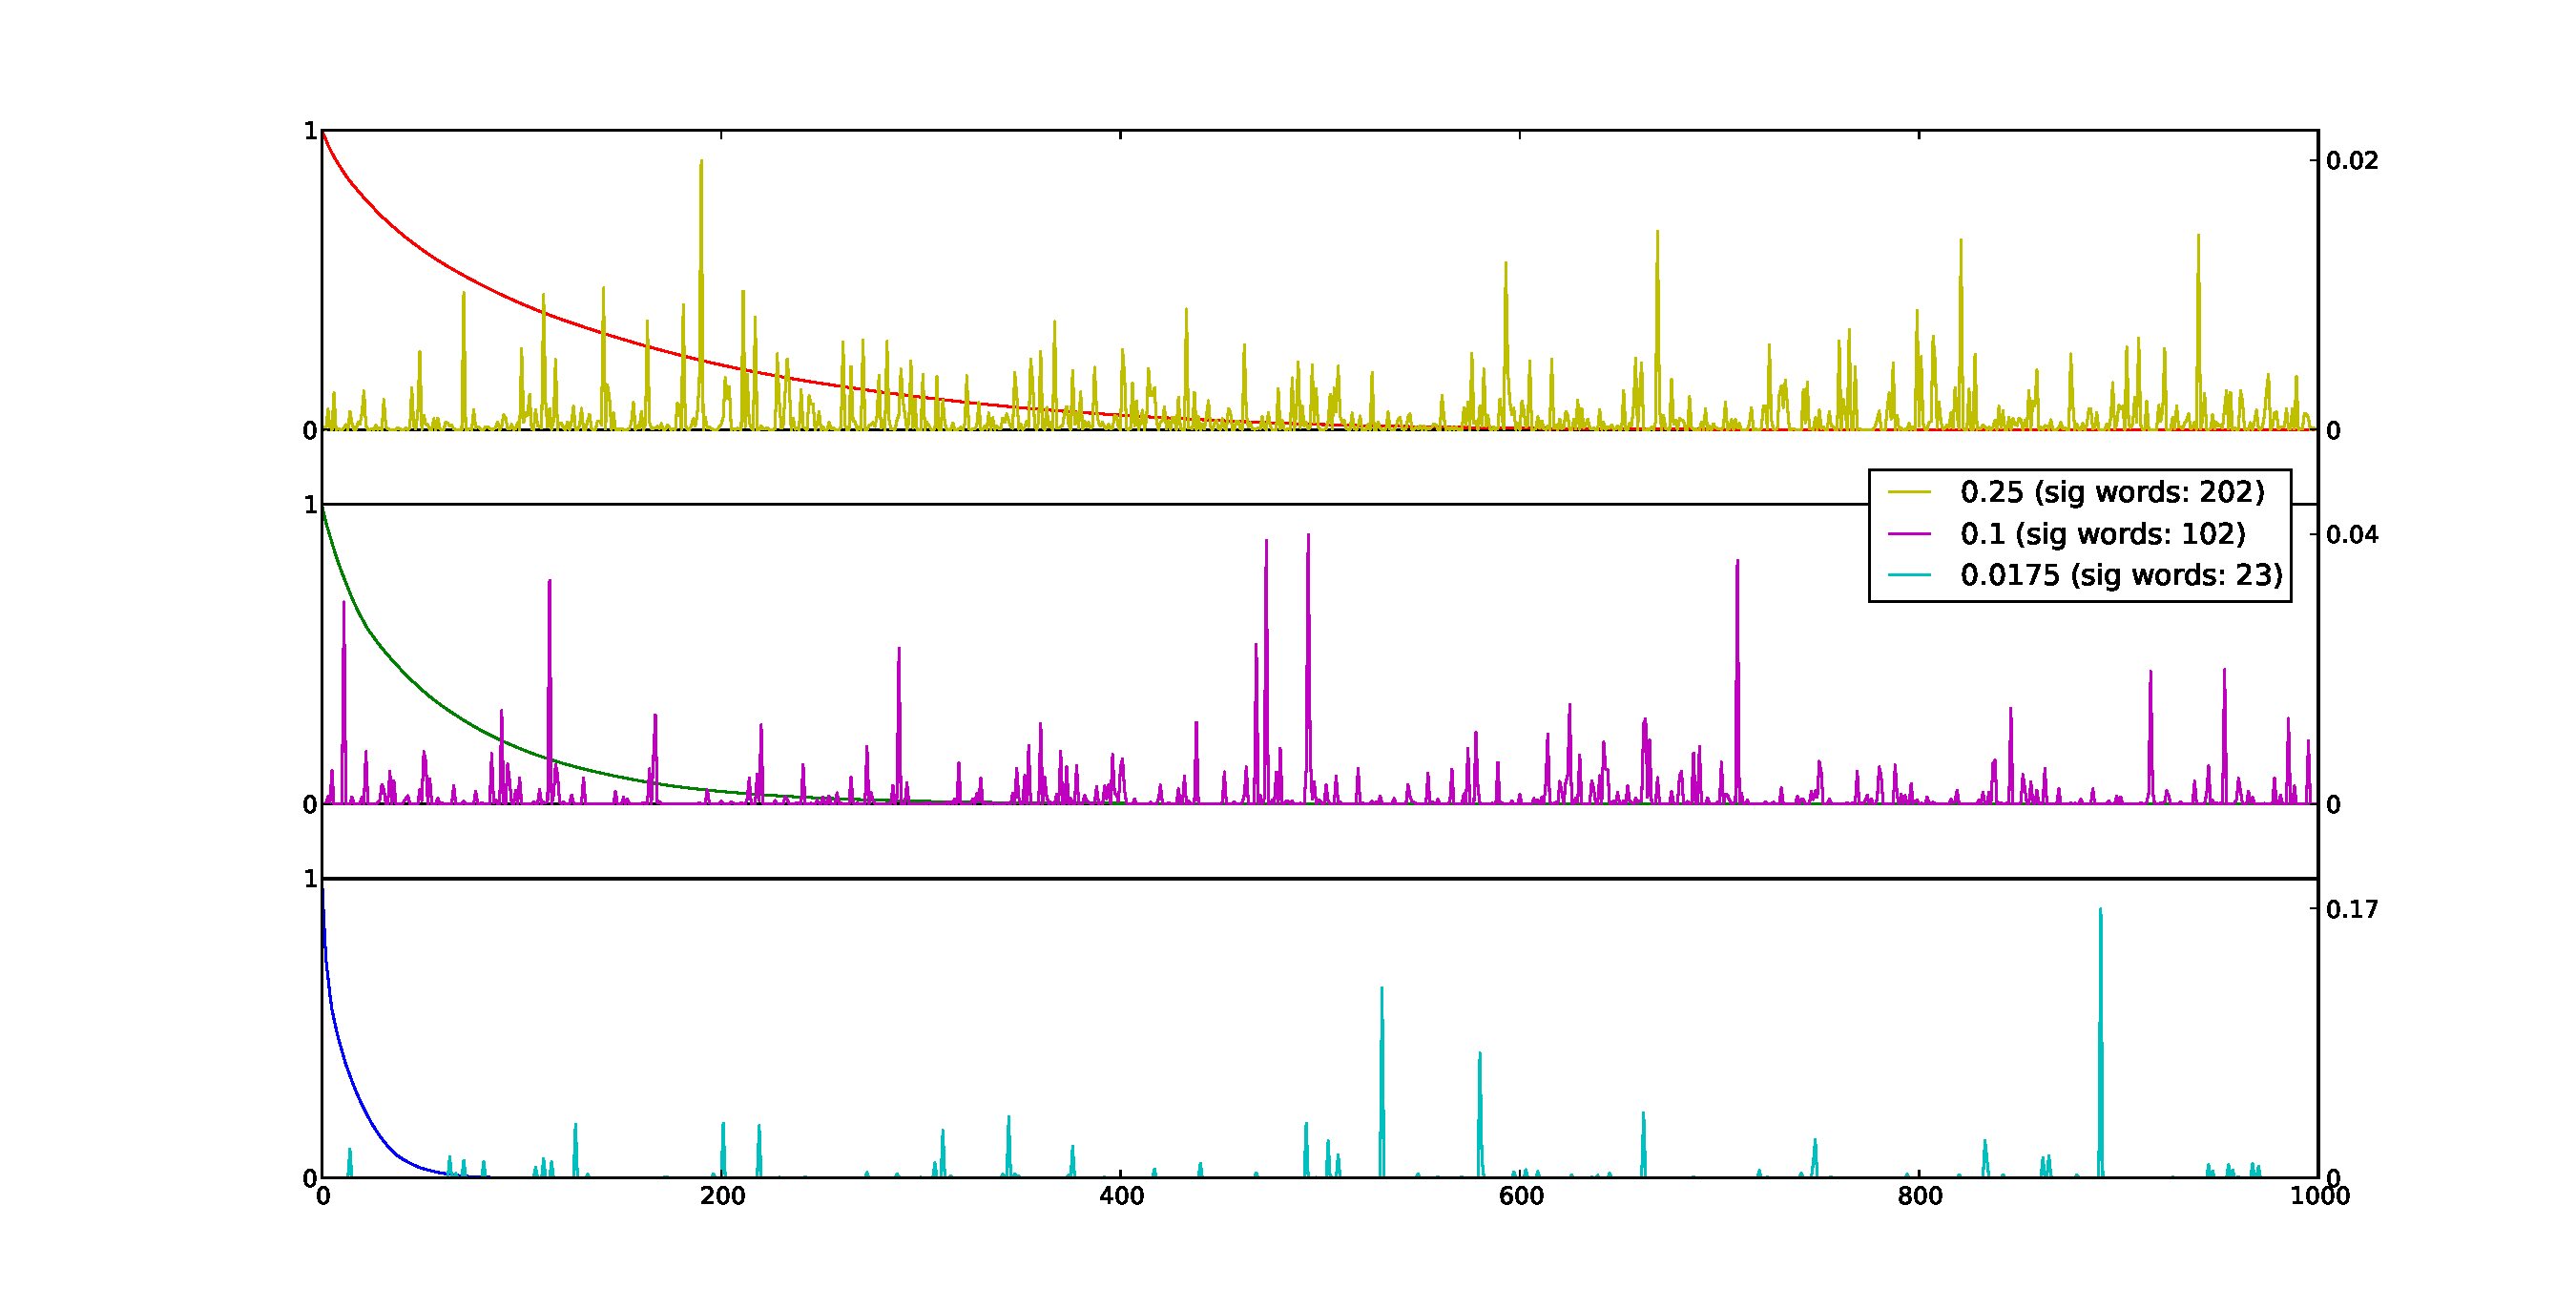
\includegraphics[width=\textwidth]{beta_plots.pdf}
	\caption{Plot of distributions on words for various $\beta$. $m=1000$, each distribution is plotted along with its cdf after sorting the words by popularity. Refer to the y-axis on the right for the scaling of the distributions. In general, larger $\beta$ values yield flatter distributions.}
	\label{fig:beta_plots}
\end{figure*} 
\setlength\tabcolsep{6pt}
To help understand the dataset, we compute the values $sig\_topic$ and $sig\_word$. For a document with distribution $\vec{\theta}$ over topics, $sig\_topic$ is the smallest $t$ such that the union of the $t$ heaviest topics in $\vec{\theta}$ has an aggregate probability of at least $0.8$. Intuitively, $sig\_topic$ is the number of significant topics of a document. Analogously, for a topic's distribution over words, $sig\_word$ is the smallest number of most popular words with an aggregate probability of at least $0.8$.Instead of using $\alpha$ and $\beta$, we use the average $sig\_topic$ and average $sig\_word$ to characterize our datasets. 

We also have collected some real world datasets.  We used the
Classic-3 datasets \cite{Classic3}, a corpus from the Associated Press
\cite{AP} pruning stop words and infrequent words, and a bag of words
dataset from UC Irvine\cite{KosNIPS}.  


\section{Experiments}
\subsection{Prediction task}
For a corpus of documents, we randomly divide the documents into the training set and the testing set, where each document is put into the training set with probability $p_t$ independently. For each document in the testing set, we hold out a certain percentage $H$ of the distinct words in the document uniformly at random. The training set is given to the algorithms. After training, each algorithm gets the testing documents, and for each document predicts $s$ terms not in the observed part of the testing document. We use the precison of the $s$ predicted terms as the score of an algorithm on a specific testing document. The score of an algorithm on the corpus is its average score over all testing documents. In our experiments, we use $p_t=0.9, H=30\%,s=3$ as our parameters.

This prediction task is widely applicable in practice, especially in
online settings with a large amount of user-generated data. A familiar
example is the collaborative filtering system by which Netflix
leverages the preferences of a large user population to recommend new
films to a customer after observing his or her viewing history. For
our purpose, the prediction task provides a more straightforward
algorithmic measure than statistical measures such as perplexity and
likelihood, which are commonly adopted in machine learning, but not
applicable to algortihms that don't reconstruct a statistical model.

\subsection{Recovery task}
For the algorithms that reconstruct a topic matrix $\hat{A}$ in the
process, we also measure how close $\hat{A}$ and $A$ are. For each
learned topic $\hat{A}_i$ and real topic $A_j$, we compute
$cos(\hat{A}_i,A_j)$, then find a maximum matching between the learned
topics and real topics. We evaluate the average cosine similarity
between the matched real and learned topics. We also carry out the
above computation using total variation distance between
distributions, and get same qualitative results between algorithms.

\section{Algorithms}
\label{sec:algs}
\subsection{Previous Methods.}

We method produces a word distribution for teach test document and
outputs the most frequently unseen words in this distribution.

\begin{itemize}

\item
{\bf Baseline:} uses the training set word distribution. 

\item
{\bf KNN:} KNN finds the $k$ most similar training documents to a
testing document, where similarity is defined as the cosine between
the two documents as vectors in the word space. For a testing
document, KNN predicts the $s$ unseen words that are most frequent in
its $k$ closest training documents. Notice baseline is just KNN with
$k$ equal to the number of training documents.


\item
{\bf LDA:} Davide Blei's implementation \cite{LDAcode} based of
variational EM uses an ``estimation'' phase to train a topic model on
the training data.  Then use the ``inference'' routine to infer a
topic distribution for a test document which than uses the topic
definitions to produce a word distribution for the document.

\item
{K-means:} Uses $k$-means with cosine similaritly to produce
a topic matrix, and uses LDA inference to produce a word
distibution for each test document. 

\item
{\bf LDA(MALLET)} Uses the implementation of LDA in Mallet
based on Gibbs sampling \cite{McCallumMALLET}

\item {\bf LDAT, LDAC} For generated LDA datasets, we have two
  "cheating" algorithms as benchmarks. LDAT knows the real term-topic
  matrix $A$ of the model and uses the ``inference'' routine to find a
  word distribution for each document.  LDAC knows the real
  term-document matrix $M$ for each testing document, and uses the
  real word distribution for a test document.  LDAC is the best we can
  do given sampling noise.

\item {\bf LSI}.  Computes the best rank $k$ subspace approximation of the document-word
matrix.  Then projects test document into the subspace to find a word distribution.

\item {\bf Projector}. We have two versions of Projector which
is described below which produces a topic word matrix.  Then
LDA inference is used on each test document to produce
a word distribution. 

\end{itemize}

%% \subsection{LSI}
%% In the LDA model, we have $M=AW$, where $A$ and $W$ are the word-topic matrix and topic-document matrix respectively. Each column of M is a probability distribution on words. The $i$th document we observe is a set of i.i.d samples from the distribution $M_i$, and we have the observed word distribution $\hat{M}_i$. In the word space $\mathbb{R}^m$, all colunms of $M$ lie in the $k$-dimensional subspace spanned by the $k$ topics $A$. The sampled document $\hat{M}_i$ will be a noisy version of $M_i$, so in the word space $\mathbb{R}^m$, the points in $\hat{M}$ will be scattered close to the subspace of $A$.

%% LSI works by computing the best rank $k$ approximation to $\hat{M}$ of the training documents
%% \begin{align*}
%% &min_{U,\Sigma,V}\norm{\hat{M}-U\Sigma V}_F\\
%% \text{such that } &U\in \mathbb{R}^{m\times k},V\in \mathbb{R}^{k\times n}\text{  } orthonormal, \Sigma\in \mathbb{R}^{k\times k}\text{ }diagonal.
%% \end{align*}
%% The optimal $U,S,V$ are computed using singular value decomposition
%% (SVD) of $\hat{M}$. LSI is not a statistical model in that the $U$ and
%% $V$ matrices contain negative entries. The subspace spanned by columns
%% of $U$ serve as an approximation of the subspace of $A$. Notice if we
%% carry out SVD on $M$, the subspace of $U$ will be exactly the same as
%% subspace of $A$.\footnote{This assumes that $k$ is the number of
%%   topics used in the LDA model which generated the data. This $k$ is
%%   provided to all algorithms. For generated data, this parameter is
%%   easy to recover in any case.} For a testing document $w$, we find
%% its projection $\hat{w}=UU^Tw$ on the subspace of $U$, and predict $s$
%% unseen words with largest entries in $\hat{w}$.

\subsection{Projector}

Projector is our new algorithm that builds upon LSI, and reconstructs
a term-topic probability matrix $\hat{A}$. The motivation is that SVD
is computationally more efficient than the LDA algorithm, and has a
clear geometric interpretation, but doesn't recover the topics as
distributions of words. We aim to start from the subspace computed by
SVD, and use some straightforward operation to construct the
topics. Our algorithm is based on geometric intuition of the documents
as points in the high dimensional word space. The algorithm is as
follows
\begin{description}
	\item[Input] $\hat{M}$: observed distributions of training documents, $k$: number of topics, $\delta$: algorithm parameter
	\item[Shift] Shift the training documents to be centered at the origin.\\
			     $center=\frac{1}{n}\sum_{i=1}^n\hat{M}_i$\\
			     $\hat{M}_i=\hat{M}_i-center\qquad \forall i=1,\ldots,n$
	\item[SVD] Compute the U, the best rank $(k-1)$-dimension approximation to the column space of $\hat{M}$\\
                                 Project all $\hat{M}_i$'s to the subspace $U$, denote $V_i$ as the projections.
	\item[Clustering] Use k-means to cluster the $V_i$'s into $k$ clusters, where in the k-means algorithm the distance between two points $x,y$ is defined as $1-cos(x,y)$.\\
				      Let $C_1,\ldots,C_k$ be the centers of the $k$ clusters (center in the sense as in euclidean distance).
	\item[Scale] Scale $C_1,\ldots,C_k$ by the smallest common scalar so that $\delta n$ of $V_1,\ldots,V_n$ are contained in the hull with $C_1,\ldots,C_k$ as vertices. 
	\item[Whitening] Make all $C_i$ distribution over words: Map all the $C_i$'s to the original word space, and then set $C_i=C_i+center$, truncate the negative entries in $C_i$ to be $0$, normalize $C_i$ so the sum of entries is $1$.\\
                                            Return $\hat{A}_i=C_i$ be the recovered topics.
\end{description}
We illustrate in figure~\ref{fig:subfigures} how our algorithm works
using the a visualization on two datasets with $k=3$
topics. Notice after the {\em Shift} step, we want to find the best
$(k-1)$-dimensional subspace since the columns from the topic-document
matrix are from the $(k-1)$-simplex.

\begin{figure}[h]
     \begin{center}

        \subfigure[$\alpha=0.1,\beta=0.25,k=3$]{

            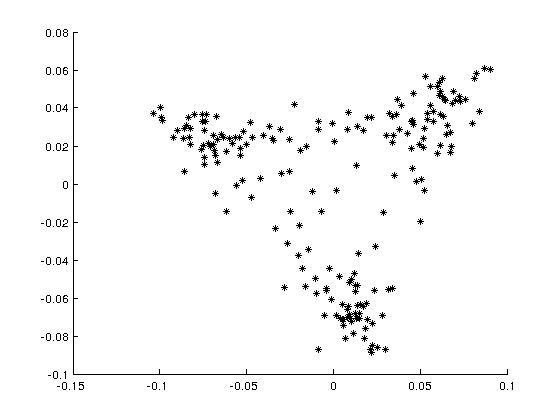
\includegraphics[width=0.35\textwidth]{c1.jpg}
        }
        \subfigure[Algorithm illustration with $\delta=0.8$]{

           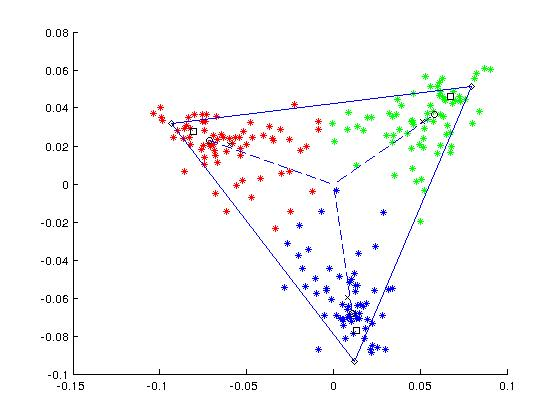
\includegraphics[width=0.35\textwidth]{c2.jpg}
        }\\ 
        \subfigure[$\alpha=0.8,\beta=0.25,k=3$]{

            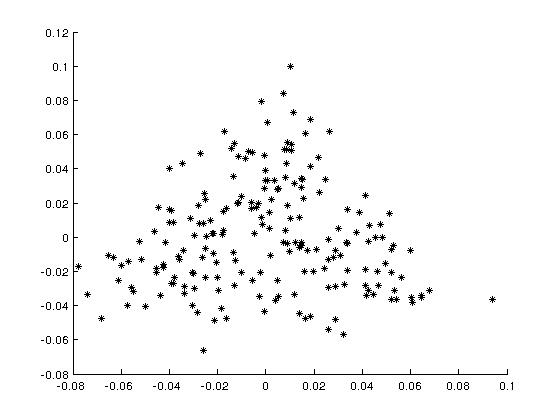
\includegraphics[width=0.35\textwidth]{b1.jpg}
        }
        \subfigure[Algorithm illustration with $\delta=0.8$]{

            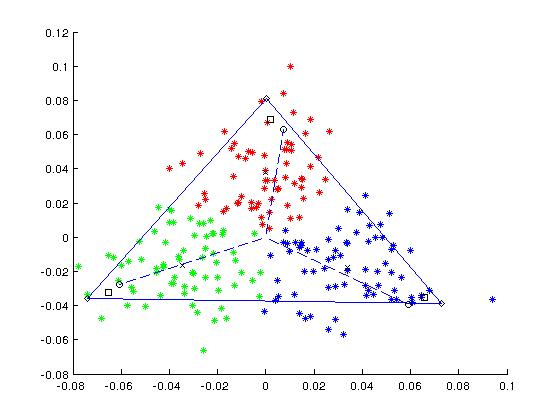
\includegraphics[width=0.35\textwidth]{b2.jpg}
        }

    \end{center}
{\small
    \caption{Illustration of Projector. The left figures are the $V_i$'s after the SVD step. In the right figures, the black 'o's at the ends of dotted lines are the real topic, black $\times$ are the $C_i$'s before scaling, black $\diamond$ are $C_i$'s after scaling, and black $\Box$ are the recovered $\hat{A}_i$'s. All points in the plot are after shifting and projected on the SVD subspace. }
}
   \label{fig:subfigures}
\end{figure}


We use estimated $\hat{A}$ and the inference procedure of the LDA
algorithm to predict words for testing documents. We use the inference
procedure of LDA since LDAT also uses it, and then we can attribute
the performance difference between LDAT and Projector to the quality
of $\hat{A}$ compared to the real topics.

We also experimented with a version of projector which does
not use LSI as a first step; it just proceeds
with $k$-means, then we project the documents into the subspace
that contains the means and scale as above.  The results
were quite similar to the results above so we do not
include them here. 

%% \subsection{Projector with $k$-means}

%% We run 

\section{Experiment Results}
\label{sec:results}
We generated datasets from the LDA model for a range of parameters,
and tested the algorithms discussed in previous section on the
prediction task. For the LDA algorithms and our Projector algorithm, we
also have results for the recovery task. We experimented with $k$ from
$3$ to $30$, and in each case, a set of $\alpha$ and $\beta$ to cover
a wide range of $sig\_word$ and $sig\_topic$. See
figure~\ref{fig:predictResult} for the prediction results of the
algorithms on a representative set of datasets.
\begin{figure}[ht]
     \begin{center}

        \subfigure{

            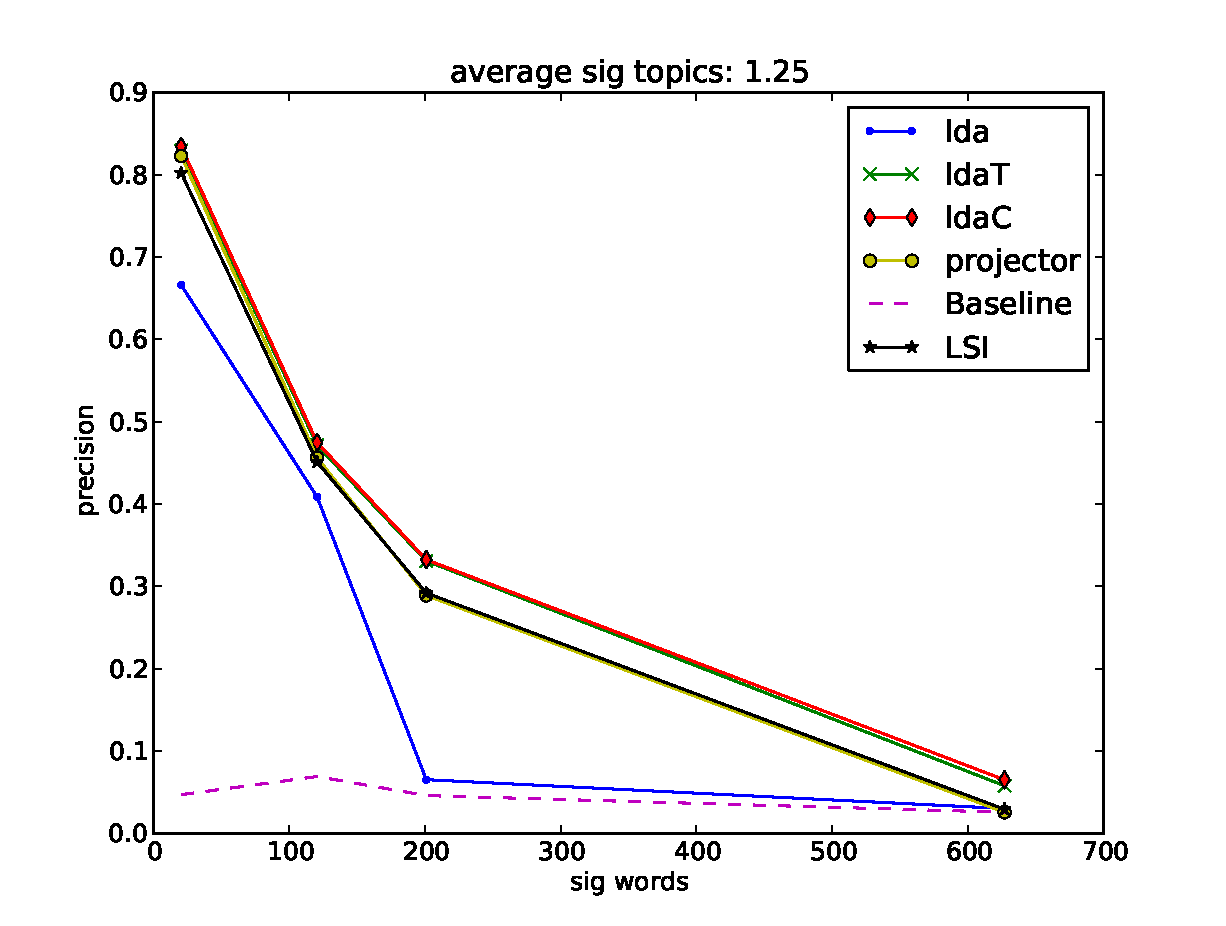
\includegraphics[width=0.1\textwidth]{k20a125.pdf}
        }
        \subfigure{

           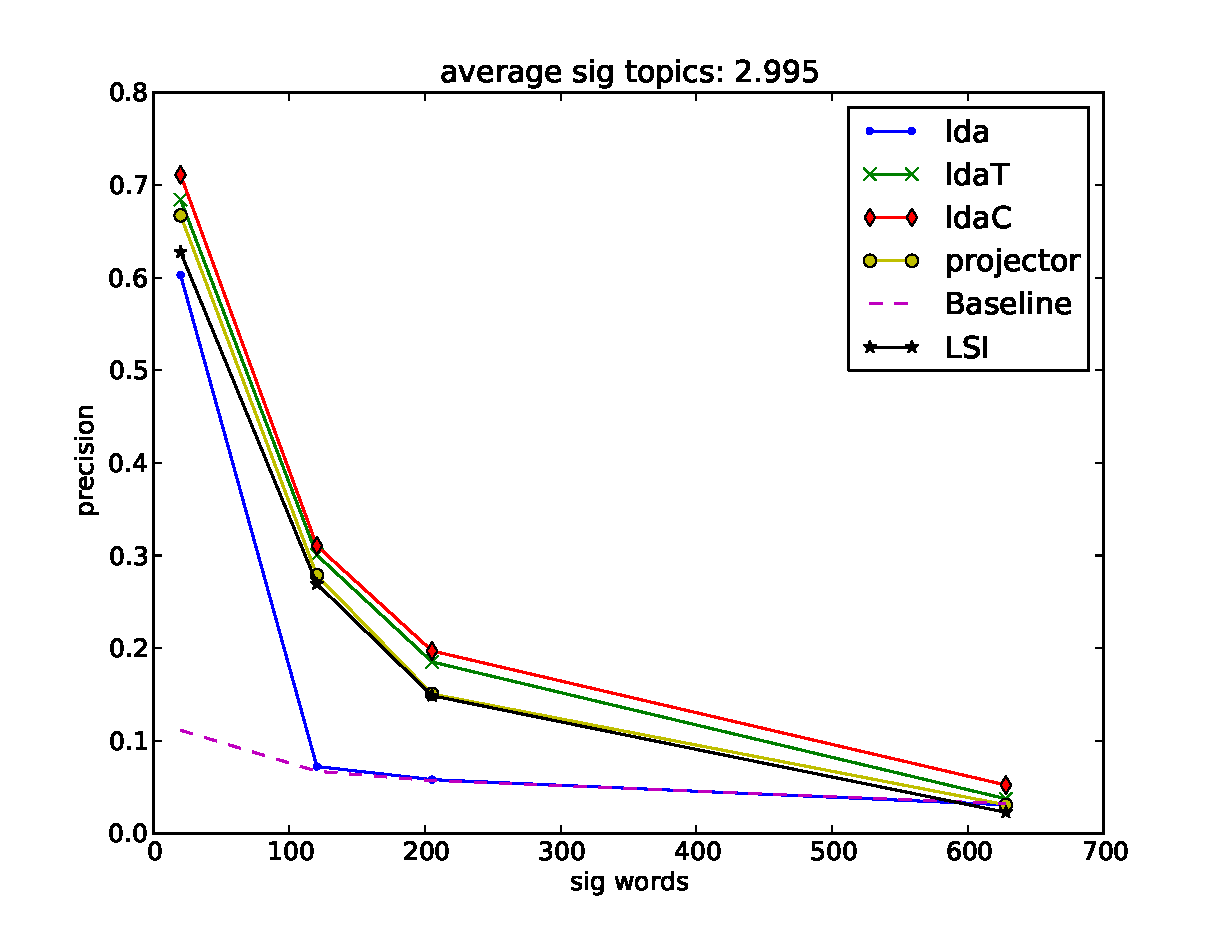
\includegraphics[width=0.1\textwidth]{k20a2995.pdf}
        }\\ 
        \subfigure{

            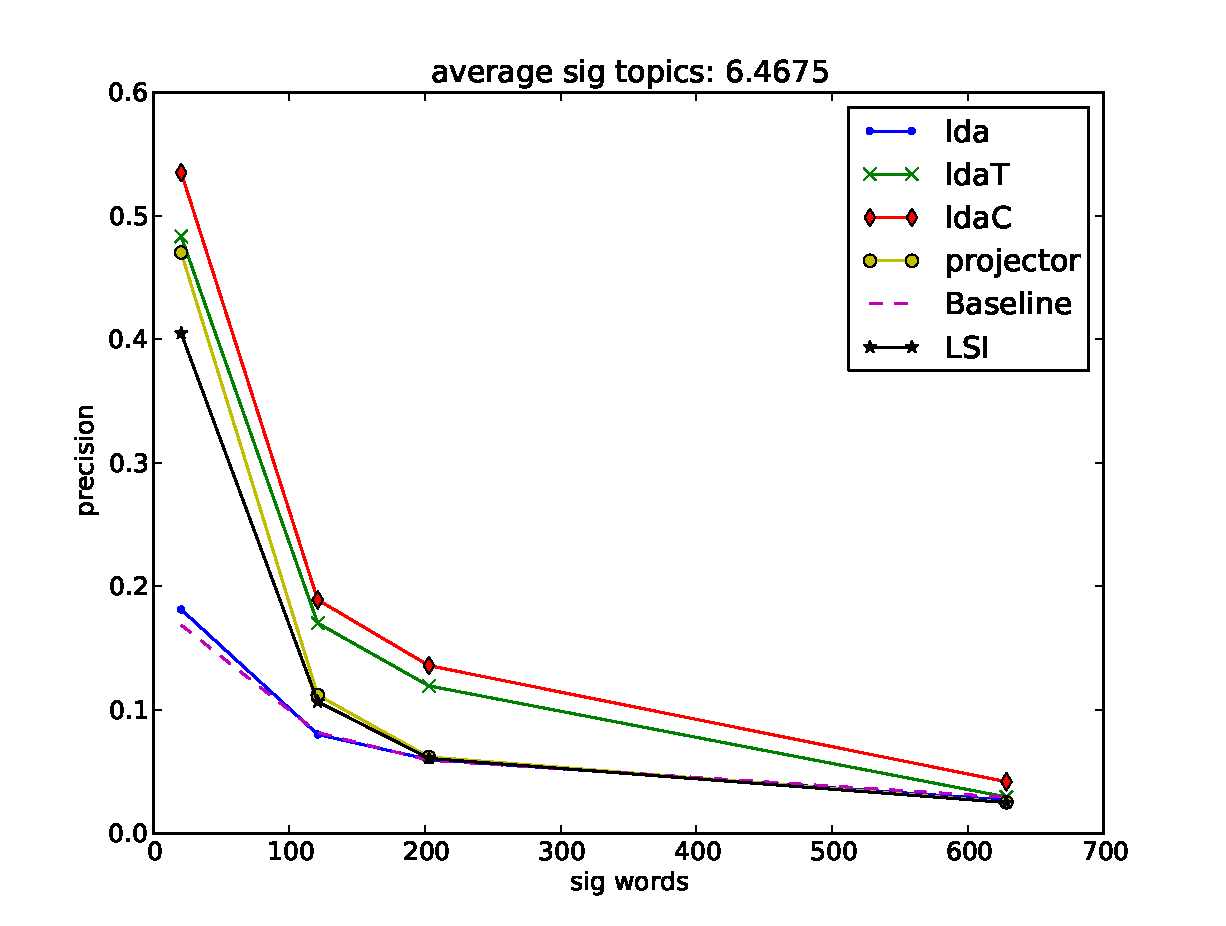
\includegraphics[width=0.1\textwidth]{k20a64675.pdf}
        }
        \subfigure{

            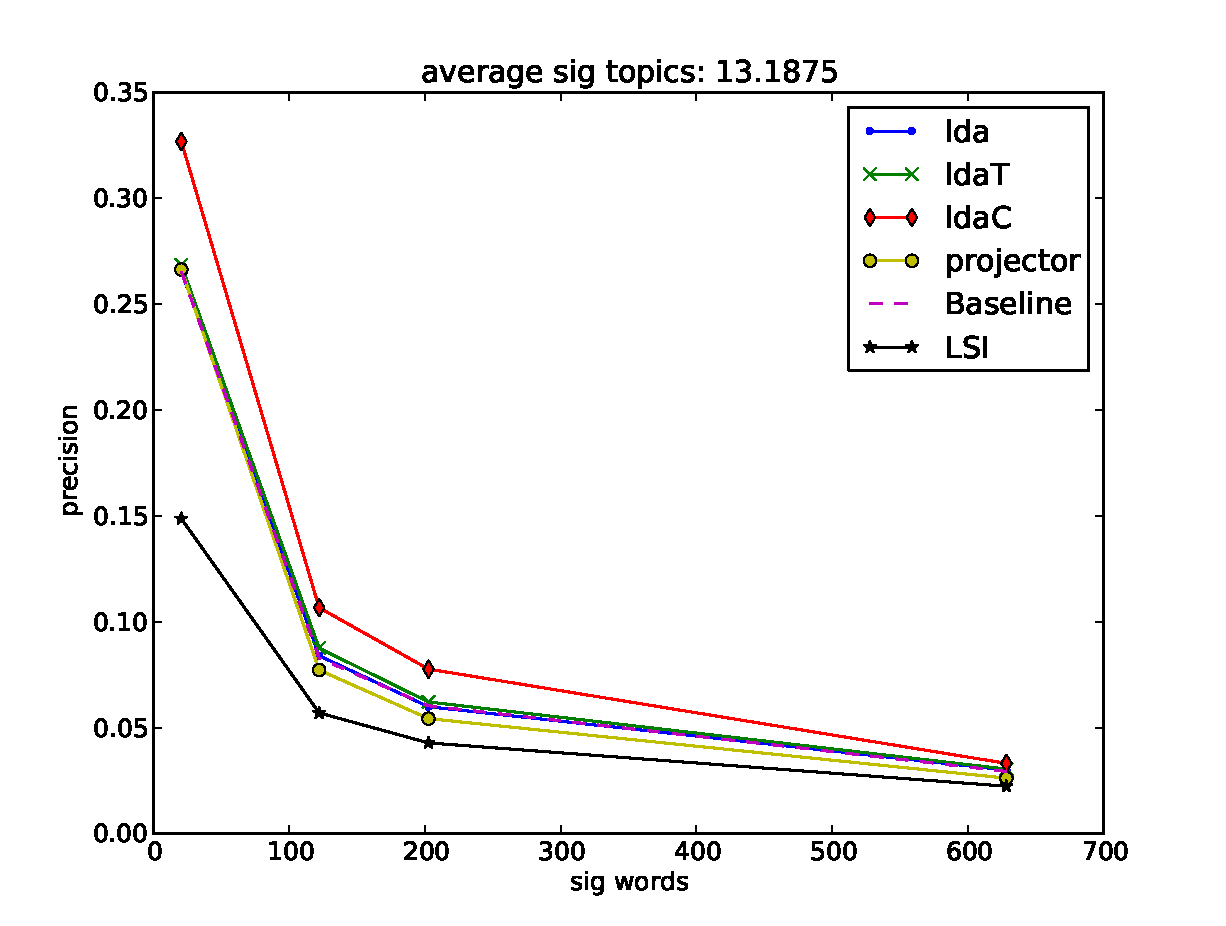
\includegraphics[width=0.1\textwidth]{k20a131875.pdf}
        }

    \end{center}
    \caption{Results of various algorithms on $16$ generated datasets, with $k=20, n=1000,m=1000,l=75$. Each subfigure has a fixed $sig\_topic$, the plots are result of the prediction task versus $sig\_word$}
   \label{fig:predictResult}
\end{figure}

\begin{table}[ht]
\begin{tabular}{|c|c|c|c|c|c|c|c|}
\hline 
 &Baseline &GibbsLda &LSI &PLSI &knn-25 &lda &projector \\
 \hline 
AP &0.14 &0.21 &0.24 &0.15 &0.25 &0.2 &0.21 \\
 \hline 
Cisi &0.09 &0.12 &0.09 &0.1 &0.14 &0.12 &0.1 \\
 \hline 
Cran &0.17 &0.21 &0.19 &0.17 &0.25 &0.23 &0.21 \\
 \hline 
Kos &0.21 &0.38 &0.26 &0.19 &0.38 &0.38 &0.3 \\
 \hline 
Med &0.08 &0.11 &0.16 &0.08 &0.17 &0.11 &0.16 \\
 \hline 
NIPS &0.64 &0.77 &0.47 &0.64 &0.75 &0.73 &0.57 \\
 \hline 

\end{tabular}
\caption{Experiment results on real datasets. We pick the result of the best among a few parameters for each algorithm. }
\label{tab:real}
\end{table}


Also see table~\ref{tab:real} for prediction results on real datasets.  There we see that
LDA is no longer dominated by LSI and Projector.  Still,  nearest neighbor's performance
dominates.  In the appendix, in table~\ref{tab:aptopics} we show the most popular
words in a sampling of topic vectors recovered by Projector in the AP dataset.

Typically, we saw the topic matching to correlate with prediction performance.
See figure~\ref{fig:size-matters} to see this result. 


\section{Analysis}
\label{sec:analysis}
%\subsection{}

In the previous section,  we defined the notion of
typical number of words in the support of a topic, or sig\_words, and
the notion of a typical number of topics in a document.  Clearly, if
both get very large one gets to a trivial topic model where each document
is generated by choosing words independently from a single probability
distribution.  

On the other hand if sig\_words and sig\_topics are small
each document should have relatively small support
compared with the corpus. Thus, in such cases we should
easily distinguish the data from the trivial topic model.

%% Here we derive an easy to compute quantity based on sig\_words,
%% sig\_topics, the total number of topics, and the corpus size to
%% predict when learning a topic model becomes difficult to distinguish
%% from the trival model.

%% Recall from the previous section, that LdaT had access included a
%% ``topic'' cheater method that knew the topic distributions while not
%% knowing anything about document topics (other than some of the words
%% in the document.)  The other algorithms were only given the actual
%% documents.

%% We wish to understand when knowing just the topic matrix is sufficient
%% and when our algorithm performs worse than the topic cheater.  We
%% compute a quantity that is reasonably predictive of both events.
%% Moreover, the point at which the algorithm performs poorly against the
%% cheater would perhaps be when the algorithm fails to learn the topics
%% well.  We examine this aspect later in this section.

We will proceed by showing that the probability of cooccurrence in
documents of two words $i$ and $j$ differs significantly from in the
trivial topic model. This can be represented as a matrix which
refer to as the co-occurence matrix.

The expected co-occurence matrix can, of course, be calculated
precisely from the topic and document distributions.  But we give
simple, even trivial, calculations that provide insight based on a
simplified topic model.

\subsection{A Uniform Topic Model.}

We proceed by calculating the difference in co-occurence matrices of a
corpus generated by a nontrivial topic model from the trivial topic
model.

Let $k$ be the total number of topics. Let $m$ be the vocabulary size. Let
$t$ be the number of topics in a document and assume that 
each word is chosen uniformly from these $t$ topics. Each topic is a
uniform distribution over $w$ words. 
%% In some sense, $t$ is a proxy for sig\_topics and
%% $w$ is a proxy for sig\_words. 
Let $l$ be the number of words in the document.

We examine word cooccurrences for $w_i$ and $w_j$: that is, the
probability that two words generated in a document are $w_i$ and
$w_j$.  Note that in a document of length $l$, there are ${l \choose
2}$ possible cooccurences between $w_i$ and $w_j$.

We compute the probability of a word cooccurrence for data from a
topic distribution versus  the trivial model with the working
vocabulary: the union of significant words in all topics which roughly has
size $v = \min(m,kw)$.

For two words from the same topic, a document contains their common
topic with probabiltiy $t/k$, and the probability that both words are
chosen is $(1/tw)^2$. Thus the probability of cooccurence from being
in the same topic is $\frac{t}{k} (1/tw)^2$.  We assume that the background
probability that the two words cooccur in the other case (or in the
case that there are no topics) is $1/v^2$.  \footnote{We note that it
is possible to set up topics so that the additional correlations one
receives in one topic are exactly cancelled out by other topics.  This
setup corresponds to coding up a parity problem in the set of topics,
but it seems unlikely to arise in any reasonable topic model.  Still,
the ``rough'' calculations here fail. Indeed, we emphasize that the
arguments are heuristic.}

When the background co-occurrence is much smaller than the
topic cooccurrence the topic model should be easy to learn.  For
example, when $\frac{t}{k}{1/(tw)^2} >> 1/v^2$ or when $1 >>
(\frac{kw}{v})^2 \frac{t}{k}$, then we should have good
performance. In figure \ref{fig:ratio}, we plot this ratio against the
performance of the projector algorithm and see that things degrade as
this value increases.


We note that technically even under the weaker condition that $tw <
v$, an algorithm could information theoretically determine the topics
with enough data but the benefit over the baseline algorithm will be
small. 

\begin{figure}[t]
%     \begin{center}
                  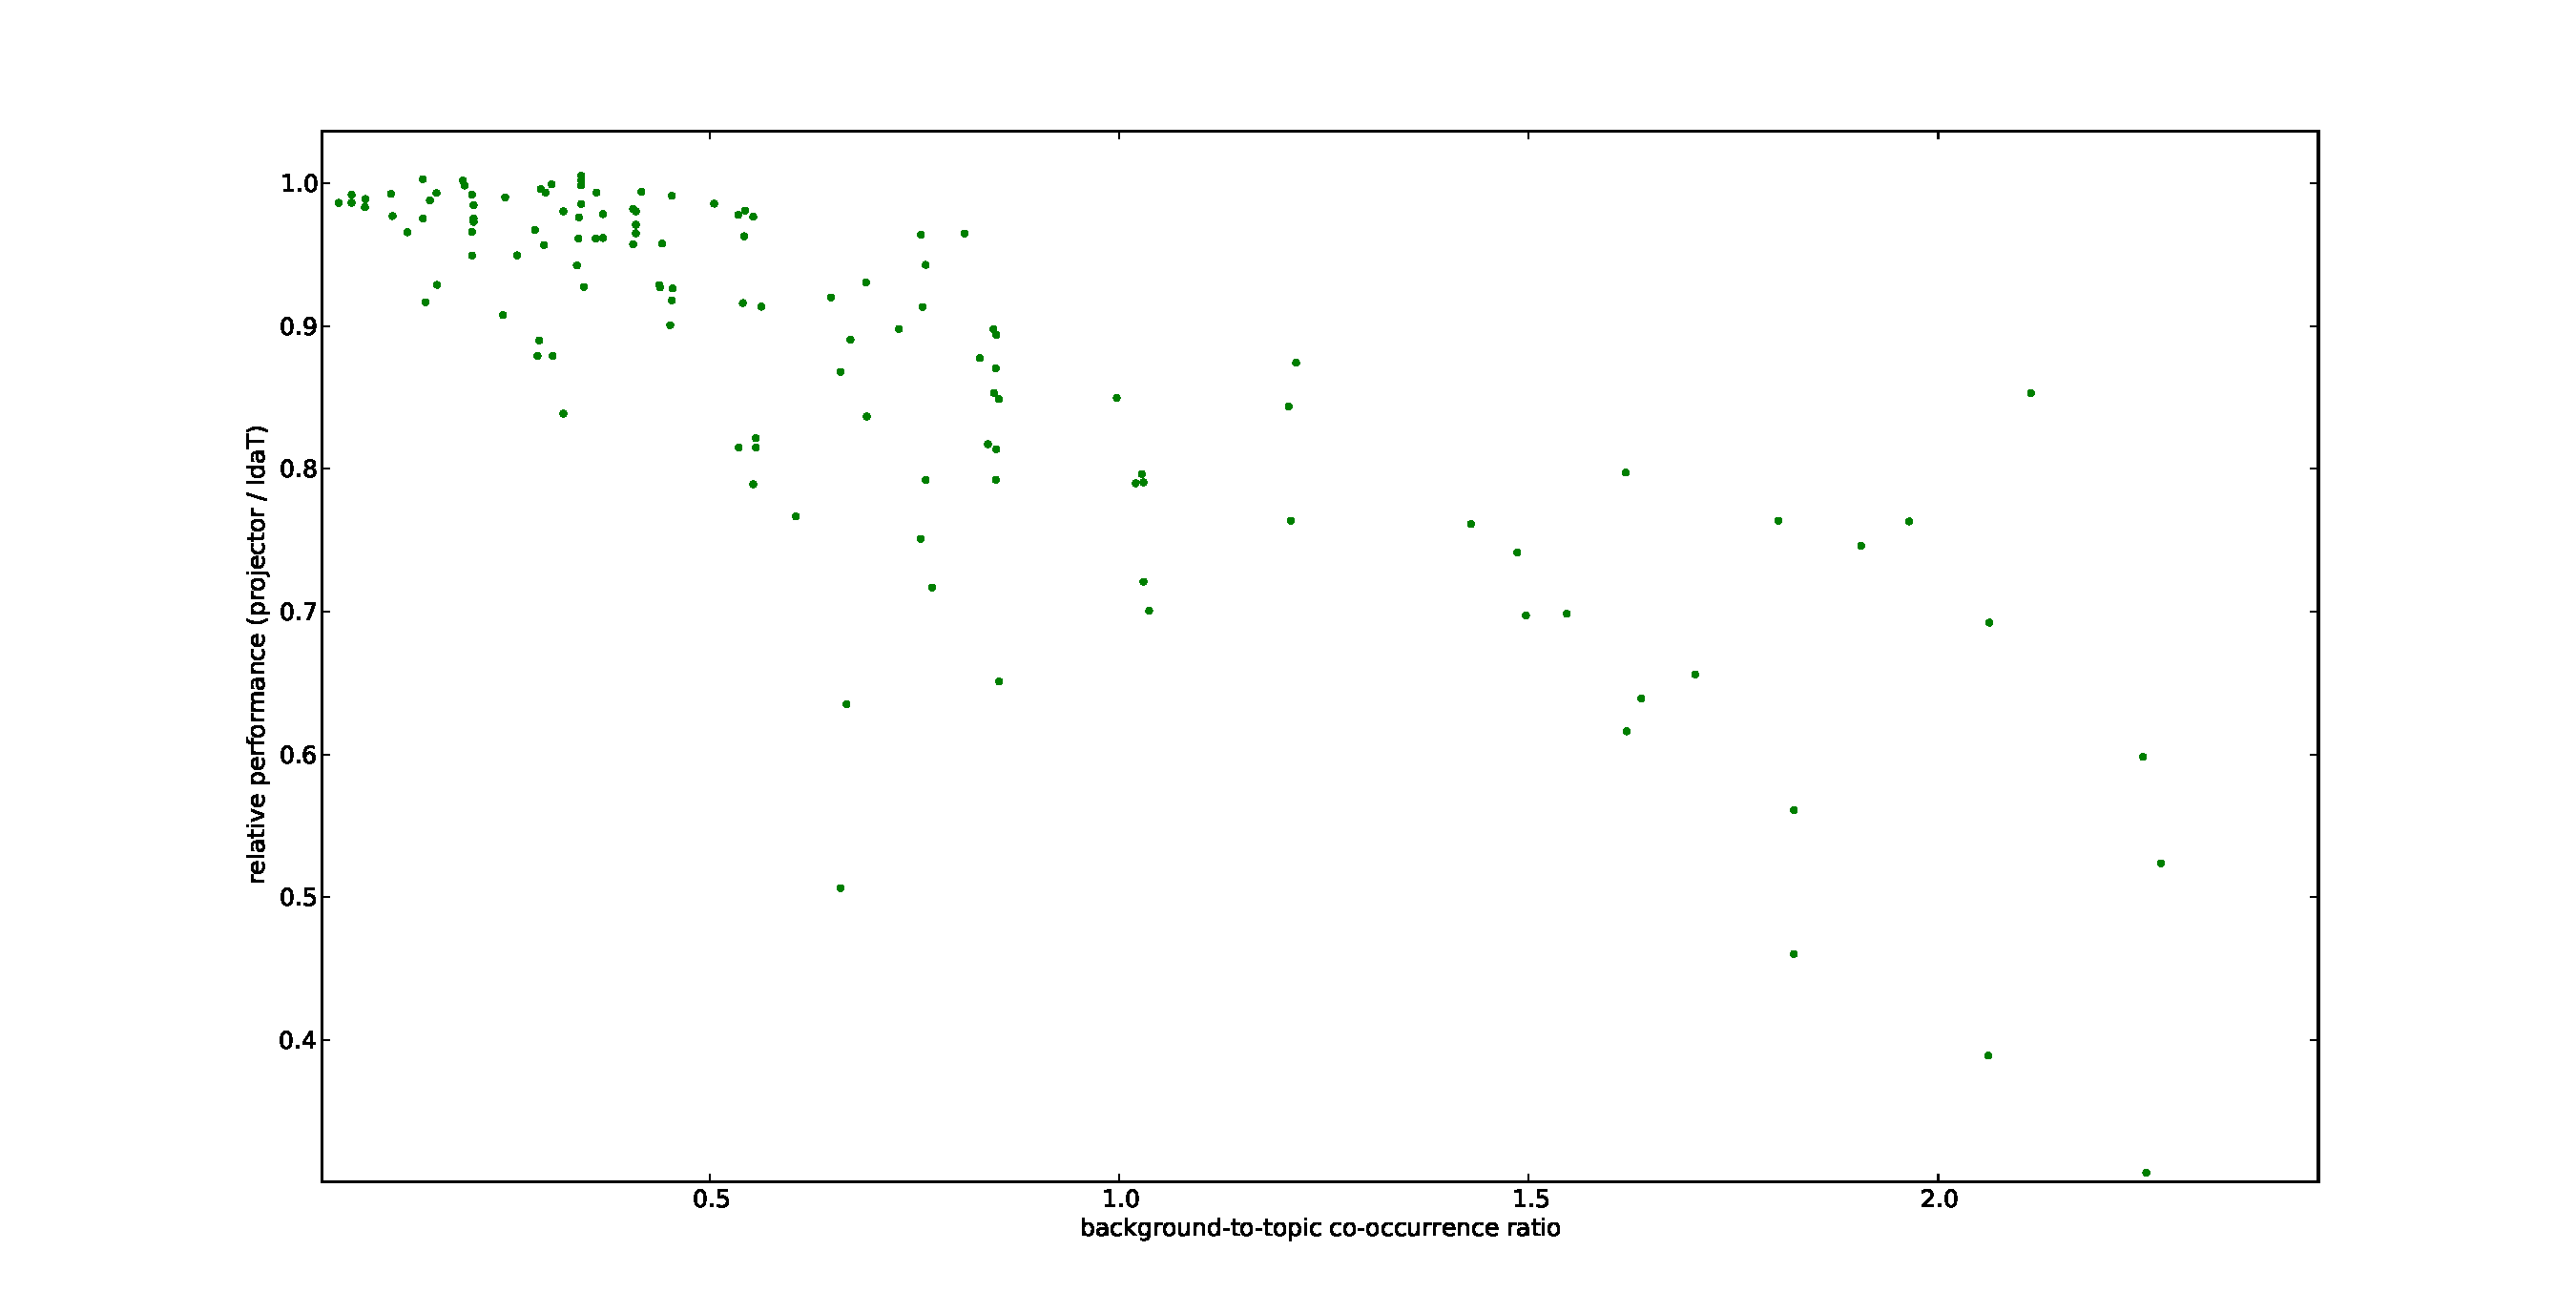
\includegraphics[width=0.58\textwidth]{projldaT-ratio.pdf}
%    \end{center}
    \caption{The performance of projector relative to LDAT falls off as the ratio of the background
to topic cooccurrences increases.
}
   \label{fig:ratio}
\end{figure}



\subsection{Dependence on document length and number.}


%% \begin{figure}
%%      \begin{center}

%%         \subfigure[]{
%%             \label{fig:a}
%%             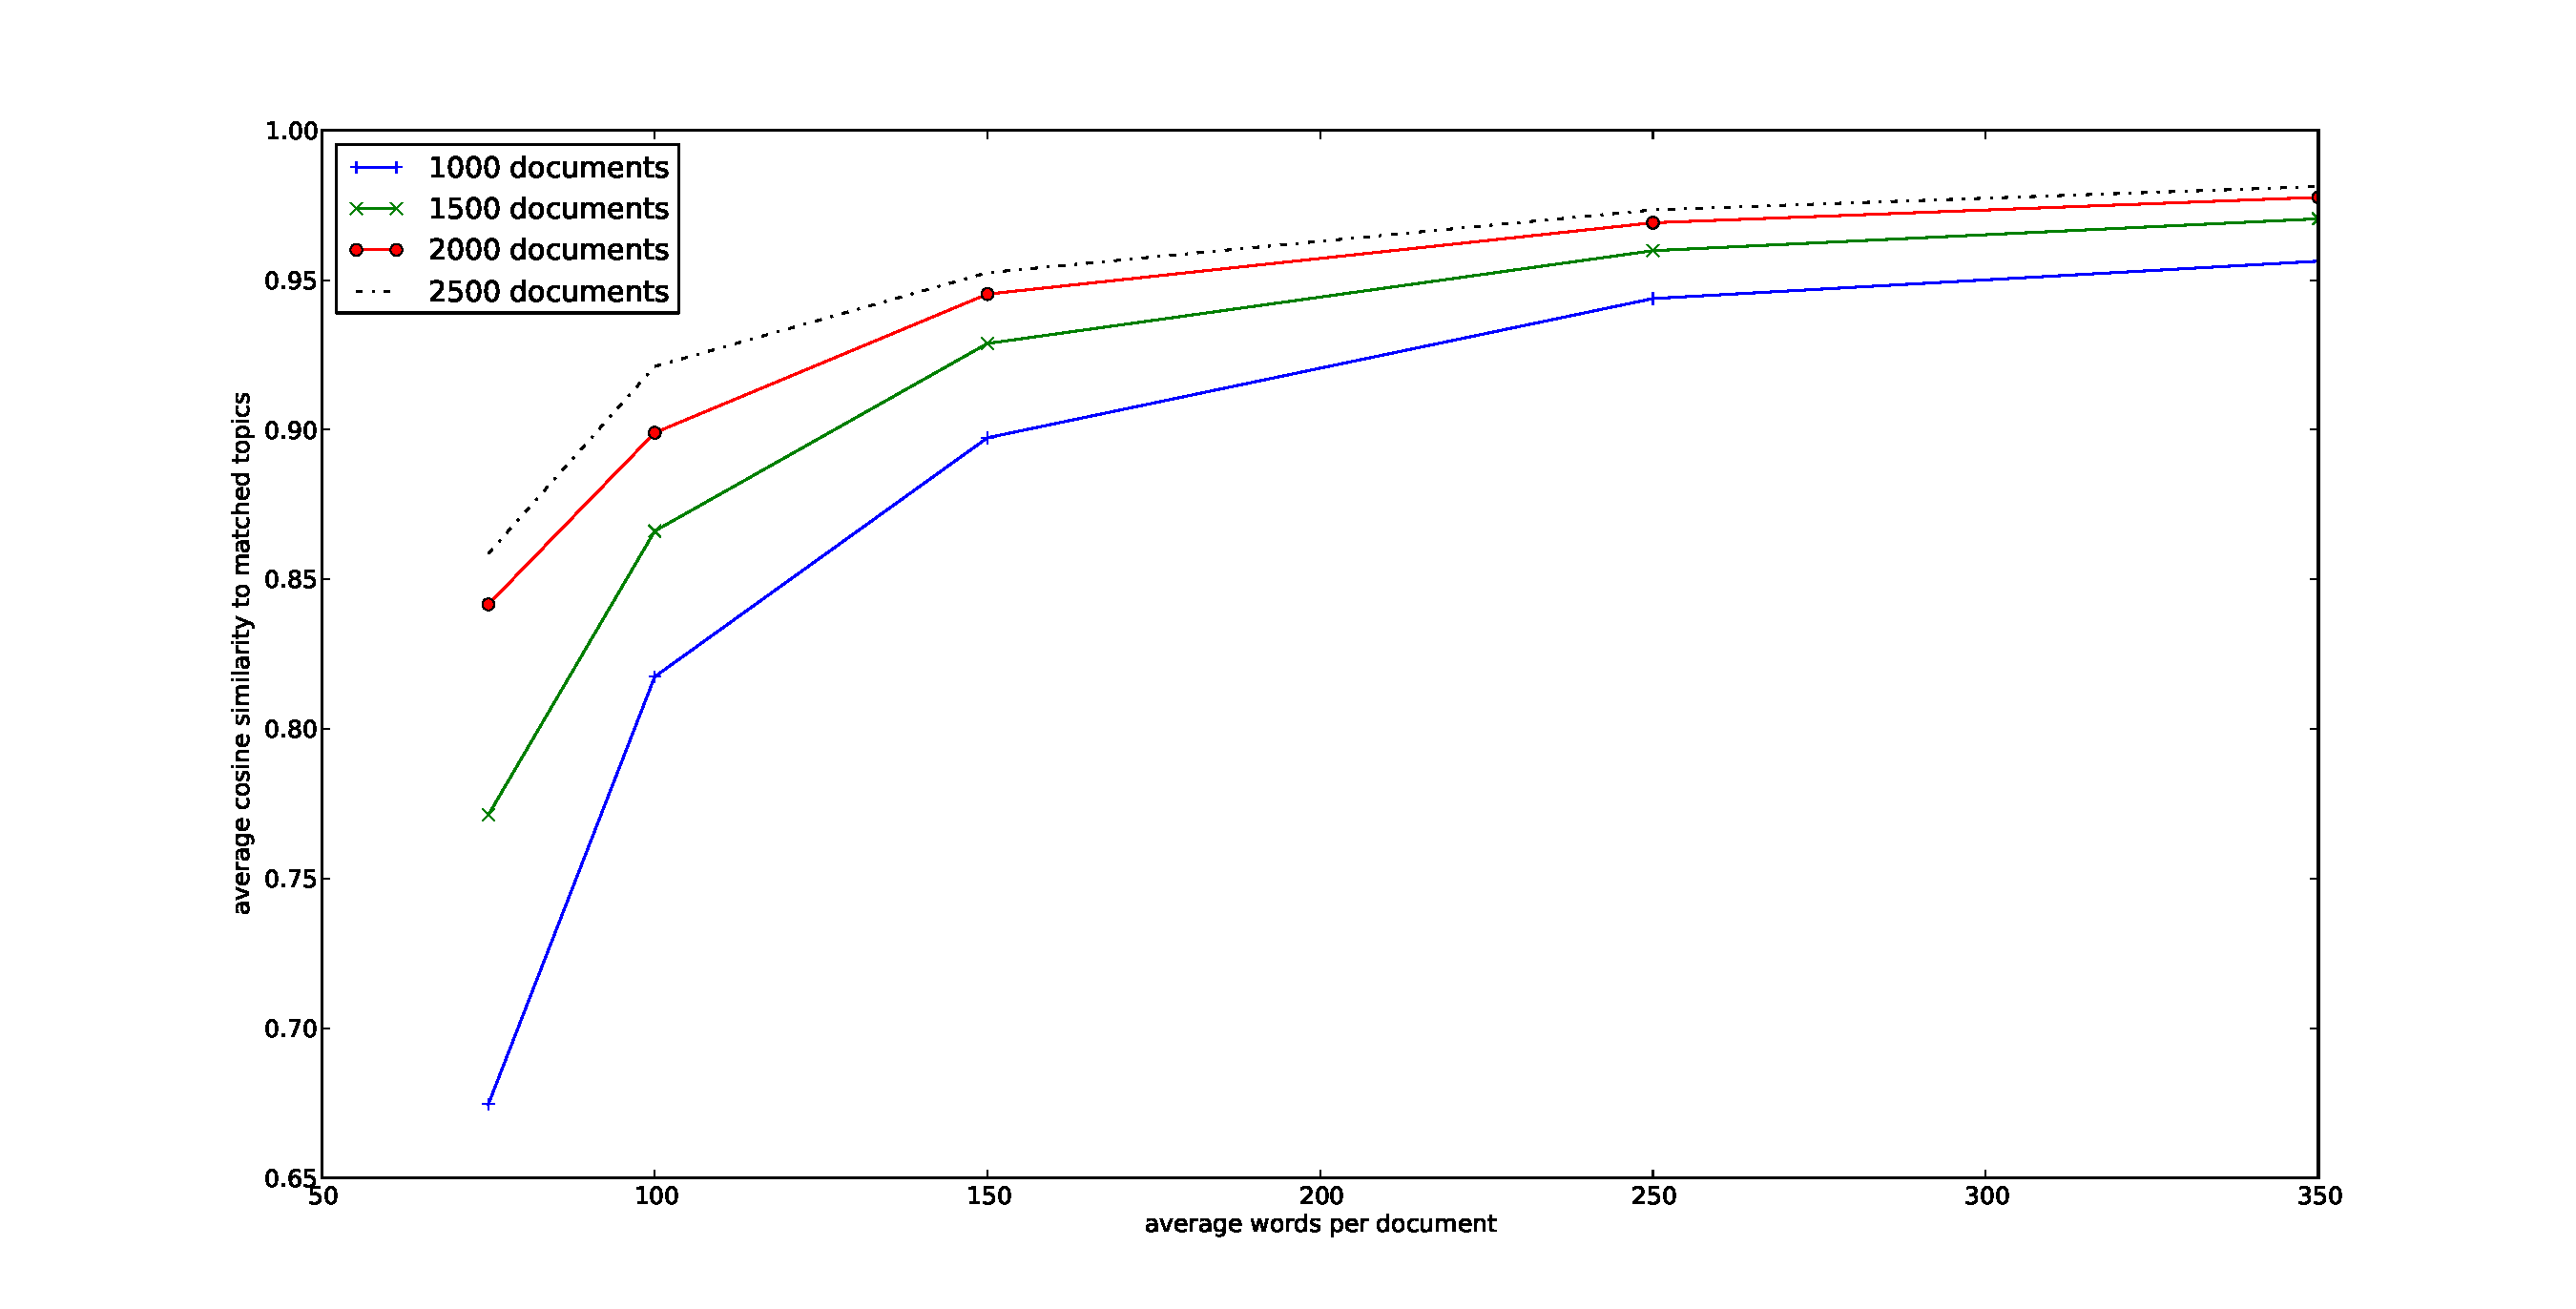
\includegraphics[width=2.5in]{projectorTopics-docs.pdf}
%%         }
%%         \subfigure[]{
%%             \label{fig:b}
%%             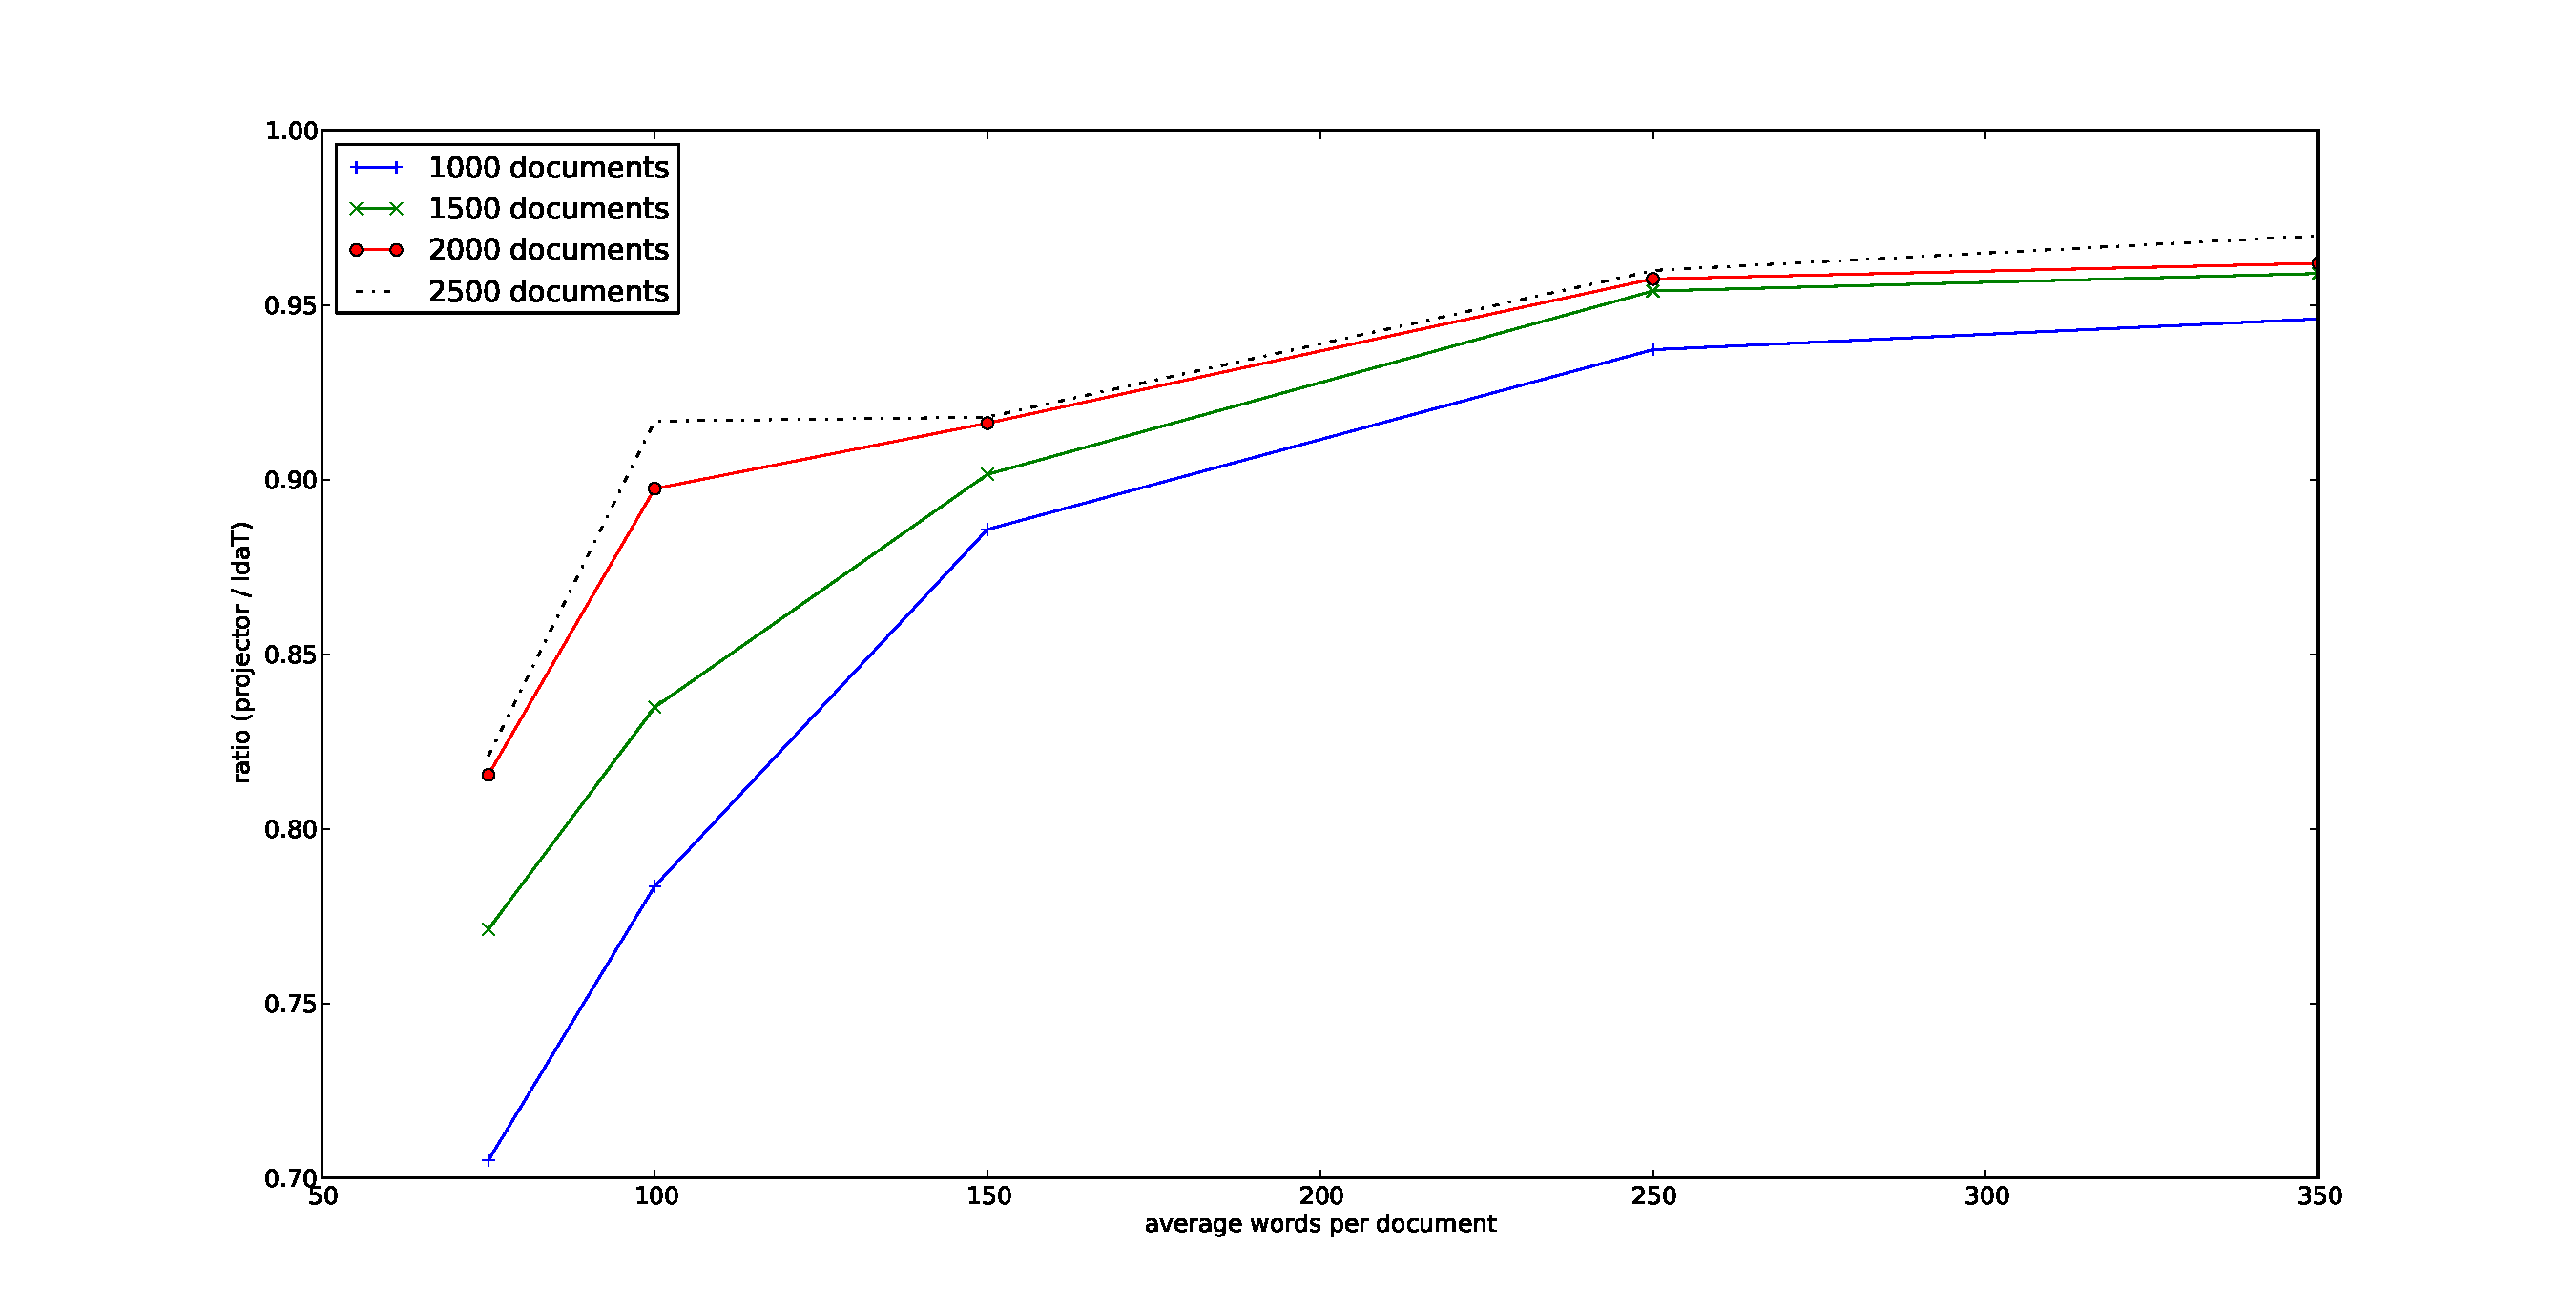
\includegraphics[width=2.5in]{projectorldaT-ratio-docs.pdf}
%%         }


%%     \end{center}
%%     \caption{Figure \ref{fig:a} above shows that as documents grow and document lengths grow, the projector algorithm
%% learns the topics better.  Figure \ref{fig:b} a corresponding increase in prediction performance comparing the LdaT algorithm that has perfect knowledge of the topics.  The different lines correspond to different numbers of documents, and the $x$-axis corresponds to the number of words in the document.}
%%    \label{fig:size-matters}
%% \end{figure}

The basic unit for determining the co-occurence values is the
number of word pairs in the corpus. The number of word pairs
grows quadratically with number of words in a document
and linearly with number of document.  This would indicate
that the performance should improve more as document length
grows as compared with document number.  We note that
the pairs inside the document are not independent but
there is an analysis that shows a nonlinear benefit.


\subsection{An external measure.}


For real world data, there is no access, of course, to the parameters
used in the discussion above. We instead use the chi squared measure
on the cooccurence matrix, $W$.  The analysis above is really just an
anlysis of the cooccurence matrix. The Chi Squared measure is defined
as $$\sum_{i,j} \frac{(W_{i,j} - E_{i,j})^2}{E_{i,j}},$$

where $E_{i,j}$ is the expected number of cooccurrences if
documents are generated from a trivial topic model with
a word distribution equal to the marginal distribution
of the data. 


\begin{figure}
     \begin{center}
            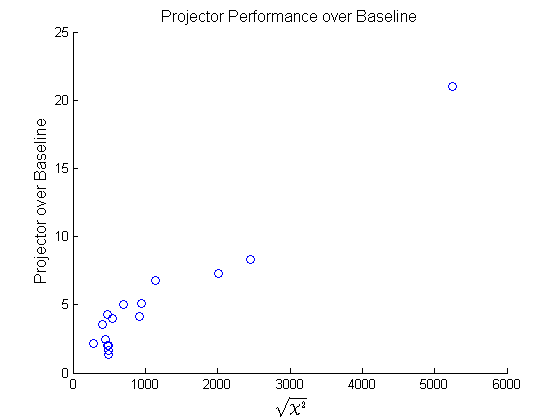
\includegraphics[width=0.45\textwidth]{x2.png}

    \end{center}
    \caption{The x-axis is the log of the Chi Squared measure on the co-occurrence matrix for the words that occur with more than average frequency. Performance relative to baseline increases with increasing Chi squared value.}
   \label{fig:x2}
\end{figure}


We remove all words for the corpus that occur infrequently and
compute the Chi-squared measure on the corresponding co-occurrence
matrix.  In figure~\ref{fig:x2}, we see that this measure 
gives us reasonable insight on the generated data
into when we get good performance on the prediction
task. 




\section{Conclusion}
\label{sec:conclusion}

In this paper, we made progress toward understanding the performance
of algorithms on data generated by the LDA model.  Using our
prediction task, we were able to find an improved algorithm for this
task.  This prediction task itself may be a reasonable candidate for
practitioners to use to evaluate algorithms that are trying to find
interesting topics. We will provide our framework either in MALLET
\cite{McCallumMALLET} or separately for this purpose.

We provided some rules of thumb for when algorithms can make
use of topic structure in generated data.  It is important
to see if these rules of thumb extend to real world datasets.
We are working on this aspect currently.

We also have begun to extend our framework to work
with hierarchical LDA, and will explore that 
in future work. 

\bibliographystyle{plain}
\bibliography{di}
\section{Appendix}

%\begin{table}[ht]
\begin{figure}
{\tiny
    \begin{tabular}{ | l | l | l | l | l |}
    \hline
    Civil Rights & Economics & Politics & Stock & Legal \\ \hline
	years & percent & states & stock & court \\
	west & rate & government & exchange & wednesday \\
	black & year & united & points & federal \\
	american & prices & union & closed & judge \\
	war & reported & war & tuesday & trial \\
	lived & increase & minister & average & convicted \\
	jr & compared & countries & tokyo & state \\
	chicago & rose & military & nikkei & death \\
	story & report & meeting & close & attorney \\
	social & higher & soviet & share & police \\
	martin & highest & leader & financial & prison \\
	progress & time & world & shares & district \\
	series & index & president & index & charges \\
	blacks & march & administration & volume & accused \\
	side & mortgages & political & timesstock & man \\
	neighborhood &  billion & forces & times & charged \\
	dream & figures & nations & million & filed \\
	king & inflation & foreign & percent & case \\
	influence & retail & prime & prices & years \\
	remains & august & capital & investors & ordered \\

    \hline
    \end{tabular} 
}
\caption{The top $20$ words (ranked by probability) for $5$ sparse topics recovered by Projector on the AP dataset. Topic names derived from top words.}
\label{tab:aptopics}
%\end{table}
\end{figure}


\end{document}
